\chapter{Implementácia}
\label{kap:implementacia}

V tejto kapitole uvedieme dôležité a zaujímavé časti z kódu aplikácie. 

\section{Autentizácia}
\label{sec:authentication}

Prihlasovanie do systému je riešené klasicky pomocou mena a hesla. Potrebovali sme
zabezpečiť, aby si účet vedeli vytvoriť iba vyučujúci. Spravili sme teda script, ktorý
vie spustiť administrátor aplikácie z terminálu. Ten si postupne pýta základné údaje,
ktoré sa po vyplnení uložia do databázy. Po prihlásení do webového rozhrania vie
užívateľ vytvárať ďalšie účty.

Pred ukladaním nového užívateľa do databázy je potrebné aby heslo bolo
bezpečne zahašované. Databázové modely definované pomocou knižnice
\textit{Sequelize} podporujú takzvané hooky. Tie sú volané napríklad
pred vytvorením záznamu v databáze, po vytvorení, pred/po aktualizovaní alebo
mazaní dát... My využívame hook pred vytvorením, ktorý nahradí heslo do zahašovanej
podoby. Na hašovanie používame funkciu \textit{bcrypt} z knižnice
\textit{bcrypt-nodejs}.

\begin{lstlisting}[language=JavaScript]
User.beforeCreate(function(user, options) {
    return crypt_password(user.password).then(function(hash) {
        user.password = hash;
    }).catch(function(err) {
        if (err) console.error(err);
    });
});
\end{lstlisting}

Po každej akcii sa aktualizuje exspirácia takzvaného \textit{session\_id} na 24 hodín
a uloží sa v databáze. Ten zabezpečuje, aby sa užívateľ mohol prihlásiť aj po
reštartovaní servera, čo sme využili pri vývoji systému.

\section{Spracovávanie dát z GTA aplikácie}
\label{sec:gtadataprocessing}

Dáta z GTA aplikácie prichádzajú POST požiadavkami na preddefinovaný
koncový bod \verb'/gta'.
Keďže sme nechceli zahlcovať kompilovaný GTA program odosielaním
týchto požiadaviek na server, potrebovali sme zvoliť alternatívu. Do úvahy prichádzali
Linuxové príkazy \textit{wget} a \textit{curl}. Na základe
porovnania~\cite{bib:curlwget} sme sa rozhodli použiť
\textit{wget}~\cite{bib:wgetmanual},
keďže na školských počítačoch nie je \textit{curl} nainštalovaný a na fungovanie
potrebuje knižnicu \textit{libcurl}, čo by znamenalo ďalšiu závislosť aplikácie.

GTA aplikácia si pri štarte spúšťa nový interaktívny bash shell, ktorý si prečíta
konfiguračný súbor \verb'.bashrc'. V ňom je nadefinovaná funkcia \verb'prompt_command'
a nastavená do premennej prostredia \verb'PROMPT_COMMAND'. Tá je volaná vždy predtým,
ako bash vypíše takzvaný prompt - v našom prípade využívame túto funkciu, keď študent
napíše nejaký príkaz do terminálu a potvrdí ho enterom. Vtedy odošleme tento príkaz na
server \textit{wget}-om.
Dáta posielame vo formáte JSON. Znaky v položke \textit{command} sme kódovali
pomocou funkcie \verb'urlencode', ktorá zabezpečovala, že znaky ako medzera nám
nepokazili fungovanie odosielania. Niektoré UTF-8 znaky boli zle kódované, čo
spôsobovalo chyby na strane servera pri spracovávaní dát funkciou \verb'JSON.parse'.
Preto sme sa rozhodli použiť kódovanie pomocou \verb'base64'.

Aby server vedel jasne rozpoznať typ dát,
je potrebné nastaviť hlavičku na \\ \texttt{Content-Type: application/json}.
Prepínač \verb'--no-check-certificate' používame na testovacie účely.
Zabezpečuje, že aj keď na server nasadíme vlastnoručne podpísaný (self-signed)
TLS certifikát, komunikácia so serverom nebude zamietnutá. V ostrej prevádzke
odporúčame tento prepínač vypnúť a používať plne platné certifikáty.
Súbor \texttt{sample\_requests.sh} obsahuje ukážky a simulácie všetkých typov dát,
ktoré odosiela GTA aplikácia.

\begin{lstlisting}[language=Bash]
 wget --no-check-certificate \
      --header="Content-Type: application/json" \
      --post-data '{"type": "start", "user": "uzivatel", \
         "hostname": "pocitac'", "date": "datum", \
         "exercise_number": "id cvicenia", "ip": "ip"}' \
      $SERVER/gta -O /dev/null
\end{lstlisting}

Pred samotným spracovaním sa kontroluje, či je IP adresa
obsiahnutá v položke \textbf{ip} povolená (sekcia~\ref{sec:gtadataprocessing:ipfilter}).
Následne sa kontroluje, či je v čase odoslania požiadavky niektorá inštancia z
cvičení aktívna
a zároveň má rovnaké \textit{id} ako to v požiadavke. Ak sú všetky tieto podmienky
 splnené, dáta sa uložia do tabuľky \textit{Post}. V opačnom prípade sa zahodia.

Okamžite po uložení potrebujeme odoslať tieto dáta všetkým prihláseným vyučujúcim.
To nám zabezpečí funkcia \verb'io.emit'. Výhodou používania Socket.io je, že si môžeme
nadefinovať vlastné udalosti. Avšak ich meno nesmie kolidovať s už preddefinovanými
udalosťami. Dáta posielame prehľadne uložené v JSON objekte vlastnou udalosťou
\verb'new_post'.

\begin{lstlisting}[language=JavaScript]
socketapi.io.emit('new_post', data);
\end{lstlisting}

Na strane klienta počúvame na túto udalosť a následne zavoláme obsluhovaciu
funkciu, ktorá zabezpečí správne zobrazenie v prehliadači.

\begin{lstlisting}[language=JavaScript]
socket.on('new_post', function(data) {
    exercise.new_post(data);
});
\end{lstlisting}

Každá inštancia cvičenia prechádza tromi rôznymi stavmi.
\begin{enumerate}
	\item \textit{scheduled} (naplánovaná)
	\item \textit{active} (prebiehajúca)
	\item \textit{done} (ukončená)
\end{enumerate}

Pri vytváraní týchto inštancií v administrátorskom rozhraní je nutné zadať
čas začiatku a konca cvičenia. Na preklápanie inštancie z jedného stavu do nasledujúceho
využívame knižnicu \textit{node-schedule}. Tá ponúka definovanie takzvaných
\textit{cronjob}-ov, ktoré sú vykonávané periodicky. My sme toto volanie nastavili
na každú minútu. Zavolá sa funkcia, ktorá preverí, či je možné preklopiť stav
niektorej z inštancií na nasledujúci.

\begin{lstlisting}[language=JavaScript]
schedule.scheduleJob("* * * * *", check_state);
\end{lstlisting} 

\subsection{Filtrovanie požiadaviek}
\label{sec:gtadataprocessing:ipfilter}

Občas chce vyučujúci zabezpečiť, aby boli študenti nútení riešiť úlohy
iba z konkrétneho miesta (napríklad učebňa v škole). Každá požiadavka z GTA aplikácie
nesie so sebou informáciu o IP adrese počítača. Na základe toho vieme určiť,
z akej siete táto požiadavka prišla. Vyučujúci si môže nastaviť povolené siete,
z ktorých bude možné riešiť cvičenie. Tieto sa dajú nastaviť v súbore
\verb'config/app_config.js' v položke \verb'allowed_subnets'.
Jednotlivé siete treba zapísať vo formáte \verb'"sieť/maska"'
(príklad \verb'"158.195.252.0/23'") a oddeliť čiarkou.
V prípade, že neuvedieme žiadnu povolenú sieť, systém automaticky prepúšťa
a spracováva všetky dáta.

Na prácu s IP adresami sme použili knižnicu \textit{ip}. Pri inicializácii
aplikácie sa pre každú povolenú sieť vytvorí inštancia
\verb'ip.cidrSubnet("ip/maska")'. Vďaka nej môžeme využiť metódu
\verb'contains("ip")', ktorá zistí, či daná IP adresa patrí do siete.
Nasledujúca ukážka demonštruje logiku kontroly IP adries.

\begin{lstlisting}[language=JavaScript]
function is_ip_allowed(ip)
{
    if (!global.ALLOWED_SUBNETS.length)
        return true;

    for (var i = 0; i < global.ALLOWED_SUBNETS.length; i++) {
        if (global.ALLOWED_SUBNETS[i].contains(ip))
            return true;
    }
    return false;
}
\end{lstlisting}

\section{Vizualizácia}
\label{sec:vizualization}

Vyučujúcemu potrebujeme zobrazovať o každom študentovi iba najdôležitejšie informácie.
Preto sme si navrhli prehľadnú \glqq krabičku\grqq ~(obrázok~\ref{img:userbox}).
V prvom riadku zobrazujeme používateľské meno študenta a pre lepšiu orientáciu
v učebni aj takzvaný \textit{hostname}, ktorý určuje meno počítača, na ktorom
študent pracuje. V pravom hornom rohu je zobrazený aktuálny názov úlohy, ktorú študent
rieši. Druhý riadok je rozdelený na dve položky. Vľavo zobrazujeme koľkými pokusmi
sa študent doposiaľ snažil vyriešiť aktuálnu úlohu. Druhá položka počíta čas od
prijatia posledného riešenia.

Neaktívni študenti sú takí, ktorí dlhšiu dobu neodošlú pokus o
riešenie úlohy. Môže to  byť zapríčinené tým, že nerozumejú zadaniu úlohy, nevedia ju
riešiť alebo len príliš dlho rozmýšľajú nad riešením. Taktiež príliš veľa pokusov
o riešenie úlohy indikuje zaseknutie alebo len drobnú chybu v riešení.
V prípade, že počet pokusov alebo čas od posledného
riešenia presahuje nakonfigurovaný limit, začne blikať červený indikátor, ktorý
upozorní vyučujúceho na zaseknutie a neaktivitu študenta v aktuálnej úlohe.
Prvotne sme počítali čas neaktivity na serveri. Uvedomili sme si, že na strane
klienta máme taktiež informáciu o čase od posledného riešenia. Preto sme sa rozhodli
nezaťažovať server a ponechať detekciu neaktivity na klientskej strane. Tam sa
periodicky každých päť sekúnd spúšťa funkcia, ktorá každému študentovi aktualizuje
čas neaktivity.

\begin{figure}[h]
	\centerline{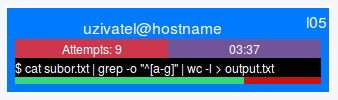
\includegraphics[width=0.7\textwidth]{images/gta_monitor_box.png}}
	\caption[Vizualizácia pokroku študenta na cvičení]{Vizualizácia pokroku študenta na cvičení.}
	\label{img:userbox}
\end{figure}

Nižšie, v riadku s čiernym pozadím, sa nachádza posledný príkaz, ktorým sa študent
snaží vyriešiť úlohu. V prípade neúspešného riešenia môže vyučujúci nahliadnuť na
tento príkaz, zistiť, kde robí študent chybu, ísť k nemu osobne a poradiť. Úplne
naspodu je ukazovateľ pokroku (progress bar), ktorý zobrazuje koľko úloh chýba
študentovi vyriešiť do úspešného konca. Jeho dĺžka sa počíta z vopred nastavenej
koncovej úlohy.

Takáto jednoduchá vizualizácia nám dáva prehľad s najdôležitejšími
informáciami, ktoré pomáhajú vyučujúcemu v lepšej a rýchlejšej orientácii medzi
študentmi na cvičení. O každom študentovi máme však zaznamenanú aktivitu počas celého cvičenia.
Kliknutím na \glqq krabičku\grqq ~sa zobrazí detailný pohľad priebehu cvičenia
konkrétneho študenta.

\section{Hodnotenie riešení}
\label{sec:evaluateexercise}

Po skončení cvičenia sa zobrazí tabuľka všetkých zúčastnených študentov s nasledujúcimi
údajmi:

\begin{itemize}
	\item Používateľské meno študenta
	\item Meno počítača, na ktorom riešil úlohu
	\item IP adresa počítača
	\item Posledná úspešne vyriešená úloha
	\item Čas strávený riešením
	\item Počet odoslaných príkazov
	\item Počet bodov za cvičenie
	\item Počet bonusových bodov za cvičenie
\end{itemize}

V tomto zozname vieme vyhľadávať a taktiež ho aj zoradiť podľa jednotlivých položiek.
Po kliknutí na jednotlivé riadky sa zobrazí okno s riešeniami študenta, v ktorom môže vyučujúci pridať hodnotenie úloh a komentár k nemu. Chceli sme tento proces
zautomatizovať a ušetriť vyučujúceho od zbytočného manuálneho hodnotenia. Pridali sme
teda tlačítko, ktoré pošle na server požiadavku automaticky obodovať riešenia.

Pri vytváraní inštancie cvičenia je k dispozícii možnosť nastavenia bodov za konkrétne
úlohy. Vzhľadom k tomu, že úloh môže byť veľmi veľa, by bolo nepraktické nastavovať
zlomok bodov ku každej jednej. Rozhodli sme sa preto, že meno úlohy bude možné zadať
aj ako regulárny výraz.
\begin{prikl}
	Majme úlohy označené ako \textit{l01}, \textit{l02}, \textit{l03}, ... ,
	\textit{l0n}. Nech za každú jednu vyriešenú úlohu je jeden bod. Potom stačí
	nastaviť regulárny výraz \verb'l[0-9]+' a počet bodov na $1$.
\end{prikl}

Algoritmus automatického hodnotenia si najskôr vyberie z databázy všetky úspešné
riešenia. Postupne sa tieto riešenia prechádzajú od najnovšieho po najstaršie.
Každé sa porovná so všetkými regulárnymi výrazmi, ktoré boli prednastavené.
Ak položka \textit{level} zodpovedá niektorému z týchto regulárnych výrazov,
potrebujeme ešte overiť MD5 haš, ktorý vygenerovala GTA aplikácia a odoslala spolu
s riešením.

Vstupmi do tohto hašu sú 3 hlavné položky: \textit{názov cvičenia},
\textit{názov úlohy} a \textit{domovský priečinok študenta}. Tie sú ešte skombinované
s písmenkami \textbf{i}, \textbf{j}, \textbf{k} a \textbf{l}. V GTA aplikácii vznikla
pri programovaní zaujímavá chyba. Pri vytvárani vstupu do MD5 hašovacej funkcie
sa očakáva názov úlohy ako celé číslo (integer). Názov úlohy je ale vždy reprezentovaný
ako reťazec znakov. Po vložení tohto reťazca do číselného formátu jazyk Go vygeneruje
výstup \verb'%!d(string=level)',
kde level je názov úlohy.
Výsledným vstupom do MD5 hašovacej funkcie je teda nasledujúci reťazec, kde operátor
+ znamená zreťazenie.

\begin{center}
	\verb'"i"' + \textit{názov cvičenia} + \verb'"j%!d(string="' +
	\textit{názov úlohy} + \verb'")k"' + \textit{domovský priečinok} + \verb'"l"'
\end{center}

Tento nami vygenerovaný haš porovnáme s tým, ktorý vygenerovala aplikácia GTA.
Ak sa rovnajú, študentovi pripočítame množstvo bodov, ktoré prislúcha
danej úlohe. Podľa toho, či je táto úloha nastavená ako bonus, tieto body pridelíme
do stĺpca \textit{bonus} alebo \textit{score}.

Takto ohodnotené riešenia je následne možné exportovať do csv súboru, ktorý je
potom ľahko importovateľný do systému Moodle, kde študenti uvidia svoje hodnotenie.

\section{Detekcia rôznych spôsobov riešenia úloh}
\label{sec:solutionclusterizing}

Fundamentálny problém, ktorý tvorí významnú rolu v rôznych disciplínach ako sú
rozpoznávanie vzorov, spracovanie obrazu, strojové učenie a štatistika, sa nazýva problém
zhlukovania. V základe je zhlukovanie definované ako problém hľadania
homogénnych skupín z danej množiny dát pomocou metódy bez učiteľa (unsupervised
learning). Každá z týchto skupiniek nesie názov
\textit{cluster}, ktorý definujeme ako región s lokálne hustejším výskytom objektov ako
v iných regiónoch.

V tejto práci sme sa rozhodli poskytnúť vyučujúcemu prehľad o
rôznych spôsoboch riešeniach úloh. Získa tak cennú spätnú väzbu o rozmýšľaní študentov
a môže prehodnotiť úpravu prednášky alebo zadaní úloh v budúcnosti. Na túto klasifikáciu riešení
sme sa rozhodli použiť metódu strojového učenia \textit{K-means}.

\subsection{K-means}
\label{sec:solutionclusterizing:kmeans}

Najjednoduchšou formou zhlukovania je rozdeľovanie jednotlivých objektov do
disjunktných podmnožín tak, že splnia špecifické kritériá. Každá z týchto množín je reprezentovaná takzvaným \textit{centroid}-om, ktorý je stredom (ťažiskom) celého zhluku.
Najrozšírenejšie kritérium je \textit{kritérium chyby clustera}, ktoré pre každý
jeden objekt spočíta jeho štvorcovú vzdialenosť od centroidu a potom vezme
súčet týchto vzdialeností pre celý cluster. Veľmi populárnou metódou, ktorá minimalizuje
túto chybu je algoritmus \textit{K-means}. Predpokladá, že objekty, s ktorými pracuje,
sú vektory. Je všeobecne známe, že táto metóda dosť
závisí od náhodného výberu centroidov na začiatku a niekedy môže vyžadovať viacero
reštartov.~\cite{bib:globalkmeans}

Algoritmus funguje v štyroch základných krokoch (vizualizácia na
obrázku~\ref{img:kmeanssteps}):
\begin{enumerate}
	\item Voľba $k$ počiatočných centroidov
	\item Každý vektor z množiny dát je priradený do clustera s najbližším centroidom
	\item Každý cluster si prepočíta nový centroid
	\item Kroky 2 a 3 sa opakujú pokiaľ aspoň jeden vektor zmení cluster alebo
		sa prekročí maximálny povolený počet iterácií
\end{enumerate}

\begin{figure}[h]
	\begin{center}
	    \subfloat[]{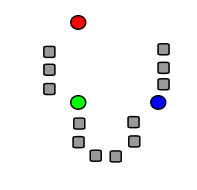
\includegraphics[width=0.23\textwidth]{images/kmeans_01.png}}
		\quad
		\subfloat[]{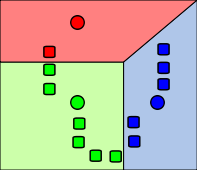
\includegraphics[width=0.23\textwidth]{images/kmeans_02.png}}
		\quad
		\subfloat[]{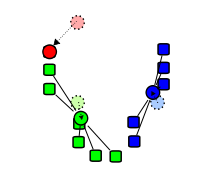
\includegraphics[width=0.23\textwidth]{images/kmeans_03.png}}
		\quad
		\subfloat[]{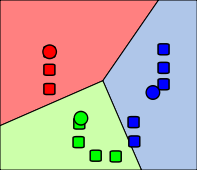
\includegraphics[width=0.23\textwidth]{images/kmeans_04.png}}
	\end{center}
	\caption[Vizualizácia fungovania K-means]{Vizualizácia fungovania K-means
		(zdroj: wikipedia, Weston.pace, licencia \href{https://creativecommons.org/licenses/by-sa/3.0/}{CC BY-SA 3.0})}
	\label{img:kmeanssteps}
\end{figure}

Najviac používané metódy pri voľbe počiatočných $k$ centroidov sú \textit{Forgyho} a
\textit{Random Partition}. Prvá spomínaná si z celej množiny dát vyberie $k$ náhodných
vektorov, kde každý bude počiatočným centroidom a pokračuje krokom tri.
Druhá priradí na začiatku každý objekt do niektorého z clusterov. \\

Formálnejšie, majme množinu dát $S=\{x_1, x_2, \ldots , x_n\}$. Nech $k$ je počet
clusterov, do ktorých chceme dáta prerozdeliť. Ďalej nech
$m_1^{(1)}, m_2^{(1)}, \ldots, m_k^{(1)}$ je $k$ náhodných centroidov na začiatku
algoritmu.\\
\textbf{Krok priradenia:}
$$S_i^{(t)}=\Big\{ x_p \mid
\forall x_p\in S~
\forall j, 1\leq j \leq k:
{d\big(x_p, m_i^{(t)}\big)} \leq 
{d\big(x_p, m_j^{(t)}\big)}\Big\}$$
kde $d$ je funkcia vzdialenosti medzi dvoma bodmi a každé $x_p$ je v iterácii $t$
priradené do práve jedného $S_i^{(t)}$ \\
\textbf{Krok prepočtu centroidov:}
$$m_i^{(t+1)}=\frac{1}{|S_i^{(t)}|} \sum_{x_j\in S_i^{(t)}} x_j$$

Na konci výpočtu dostaneme rozdelenie dát do clusterov. Je dobré vyskúšať rôzne hodnoty
$k$ kvôli presnejšej klasifikácii.
V tejto práci sme použili na klasifikáciu jednotlivých riešení
knižnicu \textit{node-kmeans}, ktorá je stabilná a má dobrú podporu. Na inicializáciu
centroidov využíva \textit{Forgyho} metódu.

\subsection{Reprezentácia vstupu}
\label{sec:solutionclusterizing:inputrepresentation}

V databáze máme uložené príkazy
jednotlivých riešení v textovej podobe. Ďalej pracujeme iba s úspešnými riešeniami.
Klasifikátor očakáva ako vstupné dáta vektory. Každý príkaz rozparsujeme na slová.
Pomáha nám v tom knižnica \textit{node-shell-quote}. V Linuxe existujú takzvané
premenné prostredia, ktoré sa pri interpretovaní volajú s prefixom \textbf{\$}.
Naša knižnica taktiež podporuje interpretovanie týchto premenných, avšak my to
využívať nepotrebujeme. Počas používania tejto knižnice sme narazili na problém,
kde regulárny výraz obsahoval identifikátor konca riadku \textbf{\$}.
Funkcia na parsovanie sa ho snažila interpretovať ako premennú. Keďže nenašla žiadnu
nastavenú hodnotu, tak túto premennú interpretovala ako prázdny reťazec, čo spôsobilo
premazanie znaku \textbf{\$}. Preto sme sa rozhodli opraviť túto chybu vo vlastnom
klone tejto knižnice a ponechávať tento znak v reťazci pokiaľ sa nenájde prislúchajúca
hodnota.
\begin{prikl}
	Majme príkaz \\
	\verb'cat file.txt | grep "^ab[0-9]+" | grep -n -o "[0-9]+" > output.txt'. \\
	Ten nám knižnica rozparsuje na nasledujúci zoznam:
\begin{lstlisting}[language=JavaScript]
["cat", "file.txt", {op: "|"}, "grep", "^ab[0-9]+", {op: "|"},
"grep", "-n", "-o", "[0-9]+", {op: ">"}, "output.txt"]
\end{lstlisting}
\end{prikl}
\noindent My si tento výstup prerobíme na množiny slov. Rozhodli sme sa pre
unigramy a špeciálne bigramy, ktoré definujeme nižšie. Používateľ si môže
vybrať, ktorú reprezentáciu vstupu chce.

\noindent\textbf{Unigramy:} Sú to slová, ktoré dostaneme z parsera. Z nich spravíme
množinu slov, v ktorej sa každé slovo bude nachádzať maximálne raz.
$$\Big\{\verb'cat',~\verb'file.txt',~\verb'|',~\verb'grep',~\verb'^ab[0-9]+',~ \verb'-n',~\verb'-o',~\verb'[0-9]+',~\verb'>',~\verb'output.txt'\Big\}$$

\noindent\textbf{Špeciálne bigramy:} Bigramy sú dvojice položiek, ktoré sa v texte
nachádzajú bezprostredne za sebou. Môžu to byť fonémy, slabiky, písmená alebo slová.
V našom prípade sa môže stať, že rovnaký prepínač
je použitý v dvoch rôznych podpríkazoch, kde zastáva rozdielne funkcionality. 
Preto sme sa rozhodli spraviť bigramy, kde prepínače a argumenty spojíme do dvojice
s príkazom, a operátory a samotné mená príkazov ostanú ako unigramy. Z hore uvedeného
príkazu v príklade teda dostaneme nasledujúcu reprezentáciu:
$$\Big\{\verb'cat',~\verb'cat file.txt',~\verb'|',~\verb'grep',~\verb'grep ^ab[0-9]+',$$
$$\verb'grep -n',~\verb'grep -o',~\verb'grep [0-9]+',~\verb'>',~
\verb'output.txt'\Big\}$$

Túto množinovú reprezentáciu spravíme pre každé jedno riešenie. Následne potrebujeme
spraviť zjednotenie slov cez všetky tieto rozparsované slová. Formálne, nech 
$R_1, R_2, \ldots, R_n$ sú množiny slov. Potom množina všetkých slov, ktoré sa
vyskytli v riešeniach je množina $R=\bigcup_{i=1}^n R_i$. Predpokladajme ďalej, že jej
prvky majú svoju pevnú pozíciu a vieme ich indexovať.

Teraz potrebujeme každú jednu množinu s riešením reprezentovať ako vektor s hodnotami
$0$ a $1$. Hodnota 1 označuje, že slovo z množiny $R$ sa nachádza v riešení
a $0$ ak sa nenachádza. Nech výsledné vektory riešení sú
$\vec{\alpha_1},\ldots, \vec{\alpha_n}$. Potom ich dimenzia je
$d(\vec{\alpha_i})=|R|$ pre každé $i=1,\ldots,n$. Každý vektor má na súradniciach
hodnoty $\vec{\alpha_i}=(a_1, \ldots, a_{|R|})$, pre ktoré platí:
$$a_j=\begin{cases}1,&\textrm{ak sa slovo z }R\textrm{ na }j\textrm{-tej pozícii nachádza v }R_i,\\
0,&\textrm{inak}\end{cases}$$

Dostali sme teda vektorovú reprezentáciu jednotlivých riešení, ktoré môžeme použiť
ako vstup do algoritmu \textit{K-means}.

\subsection{Meranie vzdialenosti}
\label{sec:solutionclusterizing:distancefunctions}

\textit{K-means} potrebuje počítať vzdialenosť medzi jednotlivými vektormi,
aby ich vedel následne rozdistribuovať do clusterov podľa najbližších centroidov.
Väčšinou sa používa \textit{euklidovská vzdialenosť}. Spočiatku sme chceli používať
\textit{Levensteheinovu} alebo \textit{Hammingovu} vzdialenosť. Tieto však pracujú
so vstupom ako celkom. Prepínače v Linuxe môžu byť rôzne preusporiadané, čo by pri
týchto metódach vypočítalo veľké vzdialenosti.
Preto sme sa rozhodli použiť \textit{Jaccardovu} a \textit{kosínusovú} vzdialenosť.
\\

\noindent\textbf{Jaccardova vzdialenosť:} Jaccardov index, taktiež známy ako Jaccardov
koeficient podobnosti, je koeficient, ktorý určuje podobnosť medzi dvoma konečnými množinami
a je definovaný ako veľkosť prieniku vydelený veľkosťou zjednotenia.
$$J(A,B) = \frac{|A\cap B|}{|A\cup B|} = \frac{|A\cap B|}{|A| + |B| - |A\cap B|}$$

Ak sú množiny $A$ aj $B$ prázdne, potom definujeme $J(A,B) = 1$.
Jaccardova vzdialenosť, ktorá meria rozdielnosť medzi množinami, je komplementárna
k Jaccardovmu indexu.
$$d_J(A,B) = 1 - J(A,B)$$

Je nutné spomenúť, že Jaccardova vzdialenosť pracuje s množinovými operáciami. Knižnica
\textit{node-kmeans} počíta centroidy priemerovaním súradníc
(viď sekciu~\ref{sec:solutionclusterizing:kmeans}). Na základe toho sme sa rozhodli
spraviť hranice, kde ak je hodnota danej súradnice väčšia alebo rovná $0.5$, slovo
patrí do centroidu, v opačnom prípade nepatrí.\\

\noindent\textbf{Kosínusová vzdialenosť:} Kosínusová podobnosť je meranie podobnosti
medzi dvoma nenulovými vektormi z unitárneho priestoru, ktorá počíta kosínus uhla,
ktorý zvierajú. Tým pádom nezáleží na dĺžke týchto vektorov.
$$C(A,B)=\cos(\theta)=
\frac{A\cdot B}{\left\lVert A \right\rVert \left\lVert B \right\rVert}=
\frac{\displaystyle \sum_{i=1}^{|R|} a_ib_i}{\sqrt{\displaystyle \sum_{i=1}^{|R|} a_i^2} \sqrt{\displaystyle \sum_{i=1}^{|R|} b_i^2}}$$

Táto podobnosť sa spravidla počíta v priestore s nezápornými hodnotami na súradniciach,
kde výsledok je ohraničený v intervale $[0,1]$. Všimnime si, že dva vektory sú si
maximálne podobné, ak sú paralelné a naopak maximálne odlišné, ak sú na seba kolmé.
Kosínusová vzdialenosť je komplementárna ku kosínusovej podobnosti.
$$d_C(A,B)=1-C(A,B)$$

Tieto metódy sme použili ako základné metriky na počítanie vzdialenosti medzi
dvoma riešeniami.

\subsection{Vizualizácia $n$-rozmerných vektorov v 2D priestore}
\label{sec:solutionclusterizing:tsne}

Pre lepšiu predstavivosť o vzdialenosti riešení, ktoré vstupujú do \textit{K-means}
algoritmu potrebujeme vizualizovať jednotlivé vektory v 2D priestore. Jediným
problémom je, že tieto vektory majú veľké dimenzie, ktoré nemôžeme priamo priradiť
na $[x,y]$ pozíciu.

Rozhodli sme sa využiť algoritmus strojového učenia \textit{t-SNE} (t-distributed
stochastic neighbor embedding) určený na vizualizáciu, ktorý
vyvinuli Laurens van der Maaten a Geoffrey Hinton. Je to technika na nelineárnu
redukciu dimenzie veľkorozmerných dát $X=\{x_1, x_2, \ldots, x_n\}$ na body v 2D alebo
3D priestore $Y=\{y_1, y_2, \ldots, y_n\}$, ktoré vieme vizualizovať.
Základom redukcie dimenzií je modelovať objekty taký spôsobom, že objekty, ktoré sú
vo veľkorozmernom priestore veľmi vzdialené ostanú vzdialené a tie, ktoré sú blízko
seba ostanú blízko. Tým máme zachovanú podobnosť.~\cite{bib:tsne}

Algoritmus \textit{t-SNE} spúšťame vo webovom prehliadači pomocou knižnice
\textit{tsnejs}.